\chapter{Temporal Dynamics\index{Temporal Dynamics}}



\textsf{ In this chapter we explain all the aspects related to Temporal Dynamics
in the NETFLIX data. We also show how to build temporal bias based model.}

\section{Temporal Dynamics in NETFLIX data}
The main goal in this work is to integrate temporal information into the
Recommender System model we are building based on collaborative filtering. It is
very important to consider temporal dynamics since the vast amounts of data we
are flooded with is dynamic in nature, and most of the information retrieval
tools today consider only the snapshot of this data, thereby loosing one very
potential dimension. In this chapter we present in detail the significance of
temporal dynamics in general and with respect to NETFLIX and also how to include
temporal dynamics into the model. \\


Since we are trying to improve the prediction rate by including temporal
effects, it is very critical to identify and uncover all possible temporal
effects within the NETFLIX data. This section summarizes and reports the
temporal analysis of the NETFLIX data.

\section{Tracking Drifting Customer Preferences}
The phenomena of $Concept drift$ is evident in the case of NETFLIX system, as we
can see that the user preferences of movies keep changing over time due to
various reasons. Concept drift means when the statistical properties of the
target variables change with time, like how user preferences change with new
release of new movies. In our case where we are trying to collaborate using
interconnected preferences among users, it is a challenge since each of the
interacting users could be drifting in different ways and also they are in
different time instances. There are mainly three kinds of approaches to include
time apect, \emph{instance selection}, in which only the recent instances are
considered, discarding off other instances. All instances within a specific time
period is given equal opportunities discarding instances ouside this period.
This obviously leads to lose of information.  In 2005, a time-weighted CF method
was proposed by Ding and Li in \cite{Ding:2005:TWC:1099554.1099689}, in
which depending on how recent the ratings are they are weighted accordingly,
these models do include time but only as weighted schemes, this is the second
approach called \emph{instance weighting}. The third approach is the
\emph{ensemble learning}, in which predictions from number of models are
combined to give a final prediction. But in this approach, if each of the
individual predoctors capture local behaviour, the global patterns are
overlooked.  A more complex approach was proposed by Koren et al, in
\cite{Koren:2010:CFT:1721654.1721677}, in
which the various complex time parameters are incorporated into the model.
We have built our model based on the following guidelines, \\
\begin{itemize}
  \item We try to model for the entire time period, instead of any particular
instances or particular time periods.
  \item We try to capture the multiple drifts based on the user, both sudden
changes and gradual changes.
  \item All the various drifts will be combined into a single framework.
\end{itemize}

\begin{example}
 As an example consider two users Joe(21 years old) and John(41 years old)
rating a common movie Godfather(1972). During November 2008, Godfather was voted
No. 1 in Empire magazine's list of The 500 Greatest Movies of All Time. Joe
after seeing this watched the movie and gave his rating. On the other hand John
had rated the movie 20 years back. This makes them both roughly the same age
when they have rated the movie, however in a different time instance. It is
clear that Joes rating could have had certain bias caused by $classical$ nature
of the movie.
\end{example}

\section{Temporal Dynamics in NETFLIX Data}
Here we would show through plots the dynamic nature inherent in the data with
respect to time. 


\begin{figure}[h]
\centering
\subfigure[Movie Means by Date]{
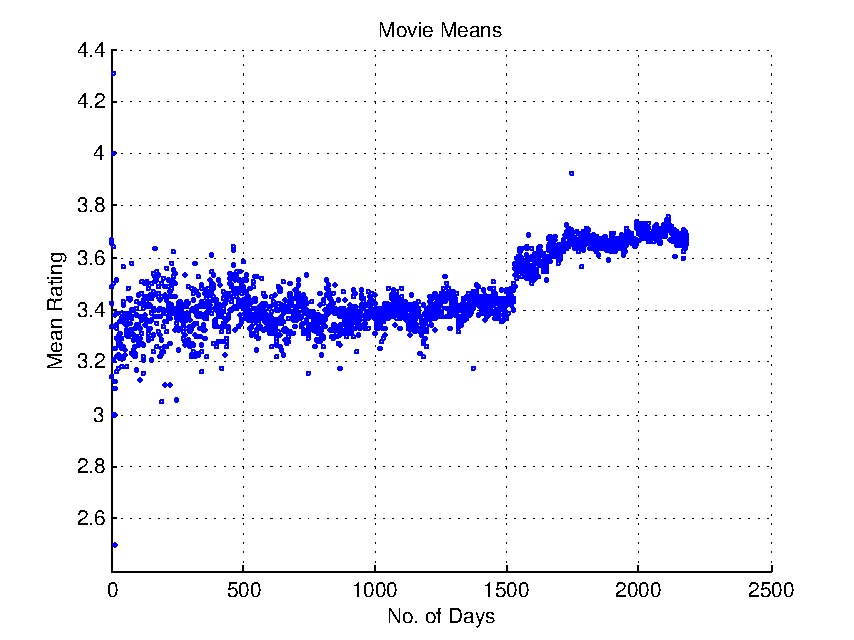
\includegraphics[width=0.45\textwidth]{./New/MovieMeans_AllMovie.pdf}
\label{fig:MovMean}
}
\subfigure[Movie Means by Movie Age]{
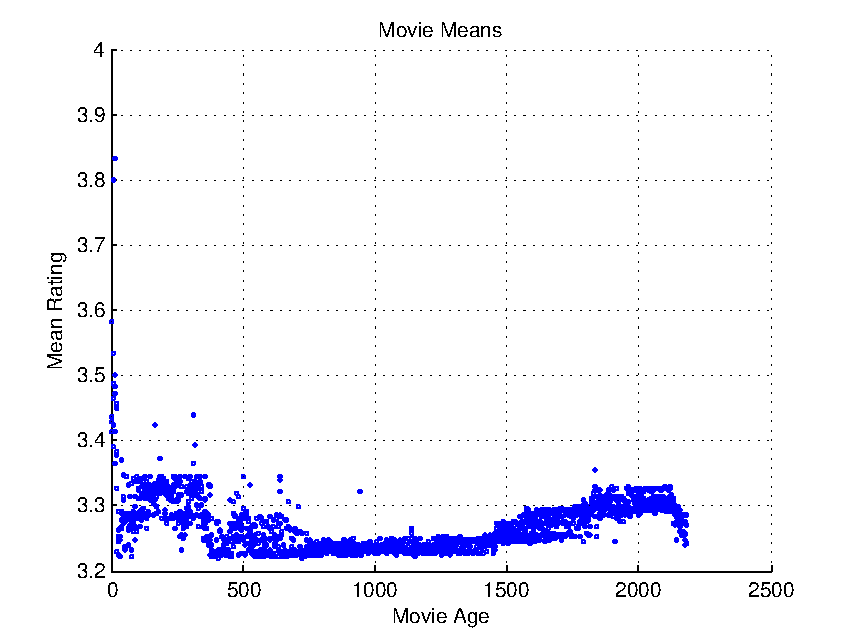
\includegraphics[width=0.45\textwidth]{./New/MovieMeans_AllMovie_Age.pdf}
\label{fig:MovMean_Age}
}\\

\label{fig:MovieMean_temporal}
\caption{Movie Means vs Time}
\end{figure}



\section{Temporal-Factor Model}
As we had seen in the previous chapter, that all the non user-item interaction
effects are encapsulated in the \emph{Baseline predictors}, we will show here
who we intend to include temporal baseline predictors. Here we explain the
theoretical analyses and findings related to various time changing aspects of
users and of movies. It is clear that the time dynamics of movies will be more
gradual than that of the users. The movies are analysed based on a large number
of users who have rated the single movie, but however as an individual user the
temporal analyses is done on large number of unrelated factors, hence the user
behaviour seems more complex and less uniform compared to the movies. \\
The main challenge is to parameterize the user-drift and the movie-drift as
appropriately as possible. The first and foremost consideration is how
transitory are the user-drift and the movie-drift. As we will expalin in detail
the movie-drift seems to be more uniform and less transient than the user-drift,
hence it is wise to consider finer time resolution to model user-drift and
coarser resolution for movies. The final model should however account for both
temporal effects spanning on a longer duration and the more transitory changes. 
For example, movies dont change on a daily basis, some of the factors which
could affect the movies dont occur often like appearance of an actor in another
movie, or the movie winning an award or the movie recieving appreciation from a
critique. On the contrary consider an user, who usually rates relative to other
ratings, so his rating scale could vary everytime he has seen on influencing
movie proir to the current movie of interest. A user who usually rate 4 for
average movies, could be influenced to rate the same kind of average movies by
3. \\

\begin{figure}[h!]
\centering
\subfigure[Monthly Average of All movies]{
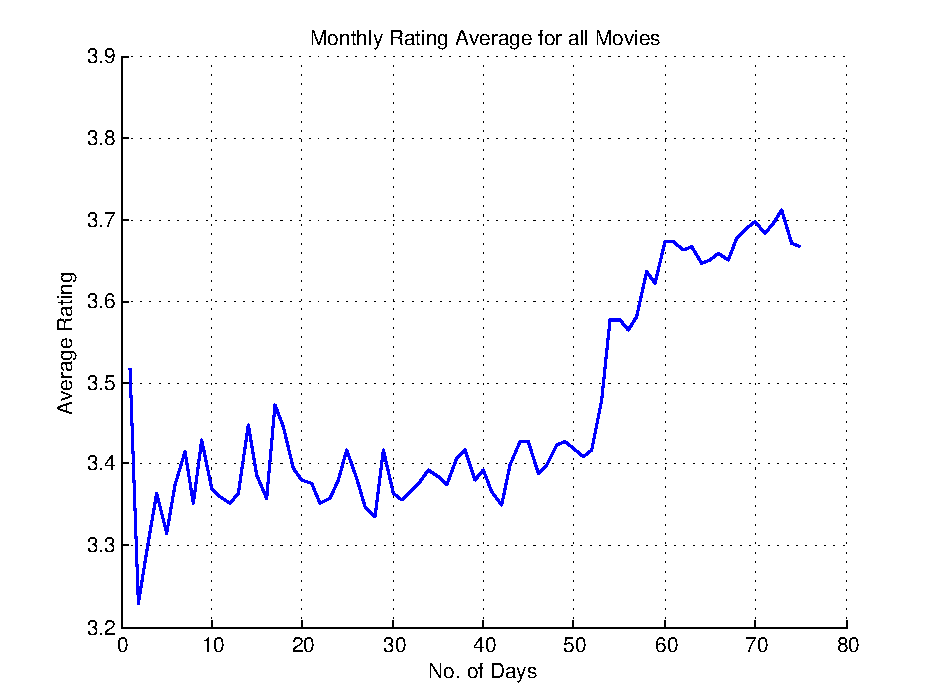
\includegraphics[width=0.45\textwidth]{./New/MonthlyAve_AllMovies.pdf}
\label{fig:MonthlyAllMov}
}
\subfigure[Weekly Average of all movies]{
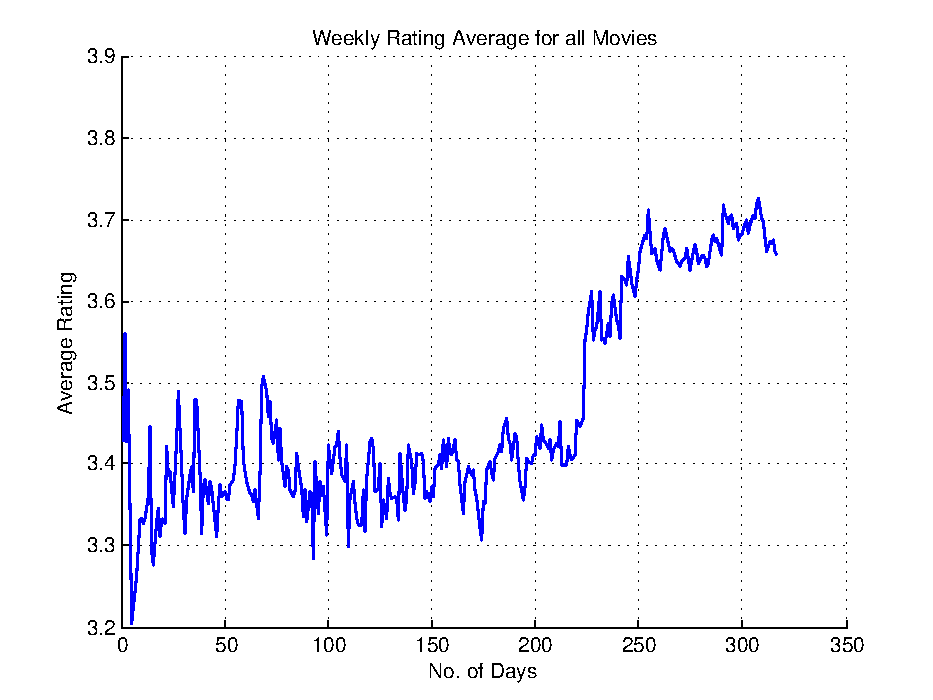
\includegraphics[width=0.45\textwidth]{./New/WeeklyAve_AllMovies.pdf}
\label{fig:WeeklyAllMov}
}\\

\subfigure[Monthly Average of movie 129]{
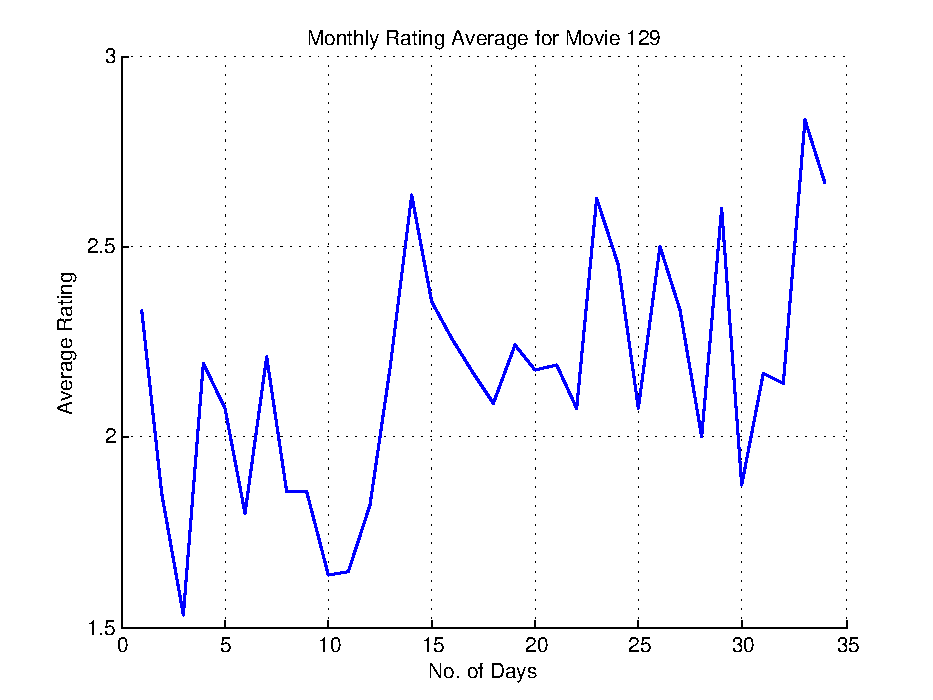
\includegraphics[width=0.45\textwidth]{./New/MonthlyAve_M129.pdf}
\label{fig:MonthlyM129}
}
\subfigure[Weekly Average of movie 129]{
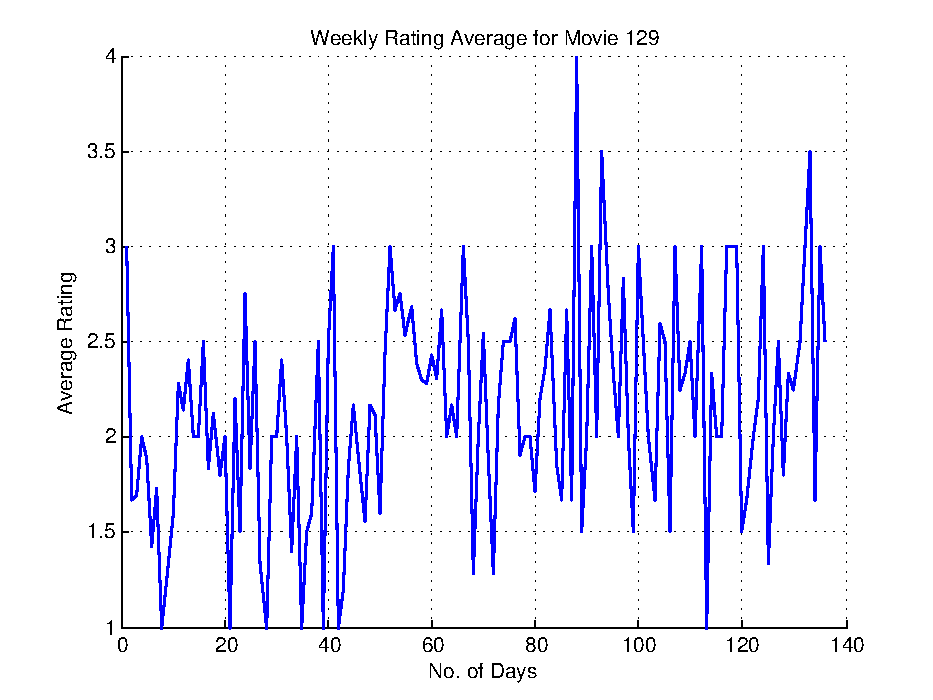
\includegraphics[width=0.45\textwidth]{./New/WeeklyAve_M129.pdf}
\label{fig:WeeklyM1476}
}\\

\subfigure[Monthly Average of movie 1476]{
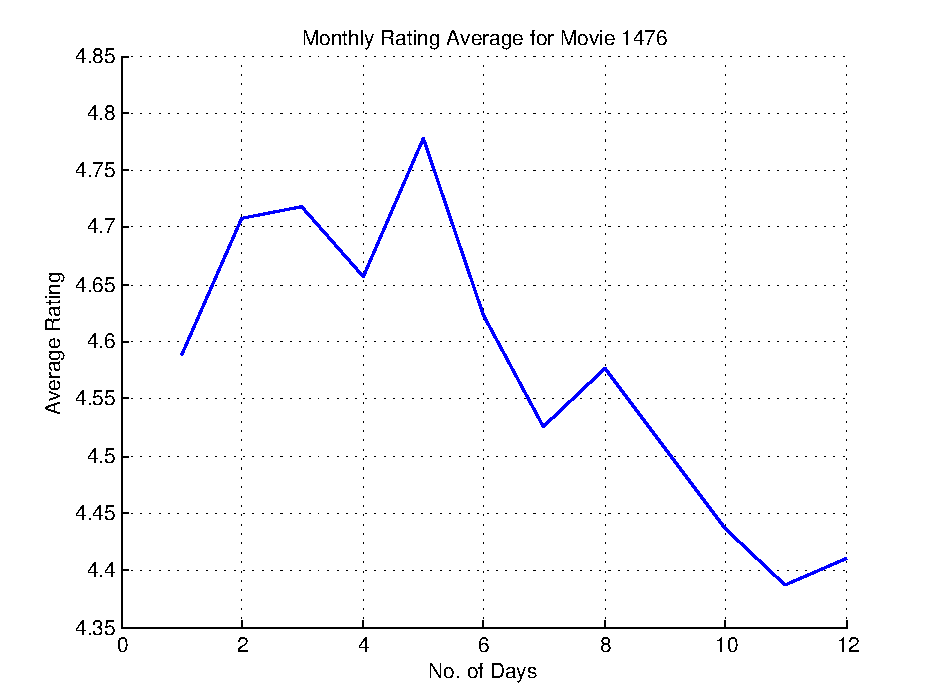
\includegraphics[width=0.45\textwidth]{./New/MonthlyAve_M1476.pdf}
\label{fig:MonthlyM129}
}
\subfigure[Weekly Average of movie 1476]{
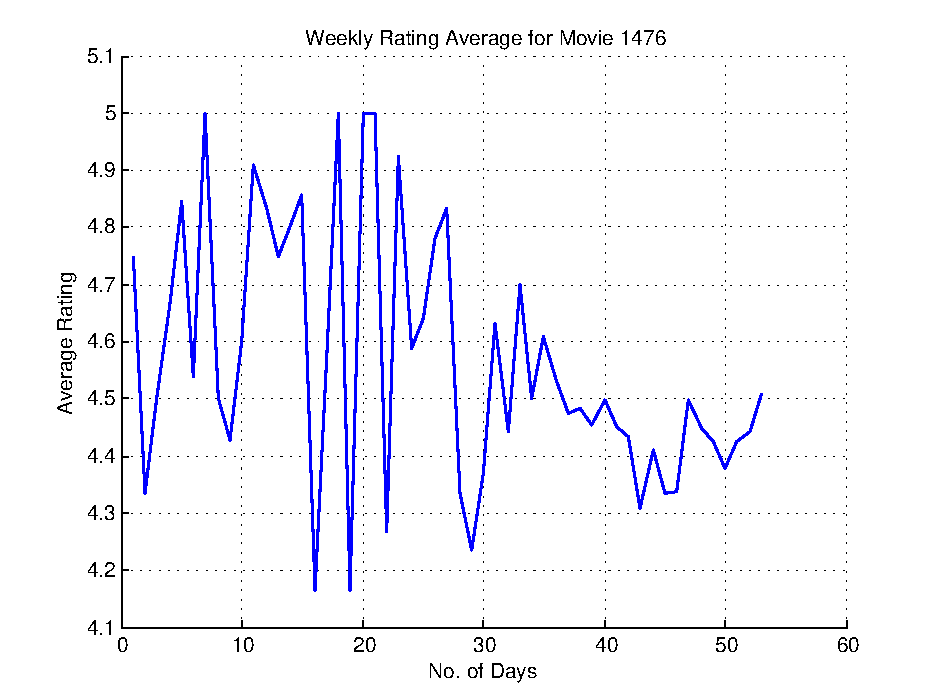
\includegraphics[width=0.45\textwidth]{./New/WeeklyAve_M1476.pdf}
\label{fig:WeeklyM1476}
}\\

\label{fig:MonthlyWeeklyAverages}
\caption{Monthly and Weekly Averages}
\end{figure}

We begun by experimenting for different time periods called \emph{bins} in order
to catch the movie-drifts.  The whole time period spans over 300 weeks, and
after several rounds of testing a 10 week period was chosen as the optimal bin
length. Hence a total of 30 bins suffice to span the entire data. With each bin
we associate it with a bias(transient part), which is simply the difference
between the overall movie mean and the mean of the movie for that bin period.
Interpolation is done for bins where there are no ratings. Each rating instance
of a movie in the training data is associated with a bin value between 1 and 30.
Hence the movie bias would have two components a stationary part, $b_{i}$ and a
transient part $b_{i,Bin(t)}$ \refname{[7]}. \\

\begin{equation} 
 b_{i}(t)=b_{i}+b_{i,Bin(t)}
\end{equation}

We have in this thesis work considered only movie related temporal dynamics,
however we would comment on a possible approach to capture temporal dynamics
related to the more complicated user bias. In case users we need to parameterize
for both long term and short term changes. A simple linear function could be
used to capture the gradual user-bias drift. Each user will have an average
rating date, and for every rating instances of this user the deviation could be
a function of the difference of the dates. Regarding sudden drifts, we need to
capture the drift on daily basis. The minimum step length could be larger than a
day also. In the NETFLIX data the user on an average rates on 40 different days,
hence we need 40 different paramaters for every user on an average. These two
factors could model the temporal dynamics of the users.  



